\documentclass[11pt]{article}

\usepackage[a4paper,margin=1in]{geometry}
\usepackage[T1]{fontenc}
\usepackage[utf8]{inputenc}
\usepackage{lmodern}
\usepackage{microtype}
\usepackage{booktabs}
\usepackage{graphicx}
\usepackage{array}
\usepackage{enumitem}
\usepackage{hyperref}
\usepackage[numbers,sort&compress]{natbib}

\hypersetup{hidelinks}
\setlist[itemize]{leftmargin=1.5em}

\title{Internal Gains Do Not Guarantee External Trustworthiness in Dermatoscopic Classification Under Simulated Label Corruption}
\author{Stelios Zacharioudakis}
\date{March 22, 2026}

\begin{document}
\maketitle

\begin{abstract}
We present TrustQueryNet, an externally validated dermatoscopic classification study under simulated class-dependent label corruption, budgeted trusted-label repair under simulated oracle supervision, post-hoc calibration, and selective prediction. The pipeline combines lesion-level HAM10000 splits, persistent noise manifests, explicit best-checkpoint evaluation, multi-seed aggregation, and external testing on the official ISIC 2019 test set. With the corrected ConvNeXt-Tiny recipe, repair reached $0.8350 \pm 0.0059$ internal calibrated accuracy and $0.7152 \pm 0.0216$ internal macro-F1 across five seeds. However, strong baselines remained close: no repair reached $0.7145 \pm 0.0130$ internal macro-F1, random repair reached $0.7105 \pm 0.0239$, and a clean-label upper bound reached $0.7330 \pm 0.0288$. On external ISIC 2019, all methods degraded sharply. Repair reached $0.5692 \pm 0.0145$ calibrated accuracy and $0.4427 \pm 0.0117$ macro-F1, versus $0.5630 \pm 0.0078$ and $0.4288 \pm 0.0123$ for no repair, and $0.5591 \pm 0.0203$ and $0.4311 \pm 0.0328$ for random repair. Internal temperature scaling did not remove external calibration fragility, and generalized cross-entropy collapsed under the chosen corruption regime. An overlap audit found zero exact duplicate images between HAM10000 and the mapped ISIC 2019 external slice. Overall, the study shows that modest internal gains from trusted-label repair do not guarantee external trustworthiness and must be judged against strong baselines, including random repair.
\end{abstract}

\section{Introduction}

Dermatoscopic lesion classification is a useful test bed for trustworthy machine learning because it combines severe class imbalance, multiple images per lesion, dataset shift across collections, and imperfect labels. The HAM10000 dataset remains one of the most common dermatoscopic benchmarks for this problem domain \citep{tschandl2018ham10000}. At the same time, clinically realistic external validation is known to be substantially harder than internal benchmarking, as highlighted by the ISIC 2019 challenge validation study \citep{combalia2022isic2019}. More broadly, calibration that appears acceptable on an internal validation split can still degrade under distribution shift \citep{ovadia2019uncertainty}. In this setting, a model can look strong in-distribution while remaining poorly calibrated or externally brittle.

TrustQueryNet was developed to evaluate these issues directly rather than treating them as secondary diagnostics. The project combines four ideas in one reproducible pipeline:

\begin{itemize}
  \item lesion-level, group-aware splitting for HAM10000;
  \item explicit class-dependent noisy-label simulation;
  \item budgeted trusted-label repair under simulated oracle supervision;
  \item calibration and selective prediction analysis under both internal and external evaluation.
\end{itemize}

This paper is not positioned as a new method paper. Its value is as a rigorous, externally validated trustworthy-ML study asking a practical question: when labels are noisy and trusted correction is budget-limited, do modest internal gains from repair survive stronger baselines and external shift?

We make three deliberately narrow contributions. First, we provide a corrected evidence slice for noisy dermatoscopic classification with lesion-level grouping, persistent corruption manifests, and explicit best-checkpoint evaluation. Second, we compare budgeted trusted-label repair against both no-repair and matched-budget random-repair baselines under a locked ConvNeXt-Tiny recipe rather than against a weak baseline alone. Third, we evaluate calibration and selective behavior both internally and externally, showing that internal confidence diagnostics do not transfer cleanly by default.

\section{Related Work}

HAM10000 provides a widely used dermatoscopic benchmark with multiple images per lesion and a clinically relevant class taxonomy \citep{tschandl2018ham10000}. For external robustness, the ISIC 2019 challenge validation study is especially relevant because it demonstrates how skin lesion classifiers degrade under more realistic distribution shift and out-of-training-category conditions \citep{combalia2022isic2019}. Our paper is positioned in that applied evaluation tradition rather than in the literature on new backbone or uncertainty architectures.

For the image backbone, we use ConvNeXt-Tiny, following the ConvNeXt architecture family \citep{liu2022convnet}. Calibration is handled with post-hoc temperature scaling, a standard and strong baseline for neural probability calibration \citep{guo2017calibration}. Selective prediction is summarized through risk-coverage analysis and AURC-style outputs, grounded in the selective classification literature \citep{geifman2017selective}. The broader uncertainty literature also warns that calibration quality can change materially under dataset shift, even when internal confidence estimates appear reasonable \citep{ovadia2019uncertainty}.

For noisy labels, the design choice here is intentionally conservative. The literature on learning from noisy labels is much broader than any single baseline family \citep{song2023noisylabelsurvey}, but this paper does not attempt a broad benchmark of robust-learning algorithms. Instead, we include generalized cross-entropy (GCE) as a practical robust-loss anchor \citep{zhang2018gce} and test whether a budgeted repair intervention beats matched no-repair and random-repair baselines. The main corrected recipe also uses light label smoothing \citep{szegedy2016inception}.

\section{Methods}

\subsection{Data and split protocol}

HAM10000 is the primary development dataset. TrustQueryNet performs lesion-level grouping so that images from the same lesion do not leak across train, validation, and test partitions. Split manifests are written to disk and reused across runs. Clean labels and observed labels are tracked separately, alongside trust and repair state.

The external dataset is the official ISIC 2019 test set \citep{combalia2022isic2019}. Labels are mapped into the HAM10000-style seven-class space:

\begin{itemize}
  \item MEL $\rightarrow$ mel
  \item NV $\rightarrow$ nv
  \item BCC $\rightarrow$ bcc
  \item AK $\rightarrow$ akiec
  \item SCC $\rightarrow$ akiec
  \item BKL $\rightarrow$ bkl
  \item DF $\rightarrow$ df
  \item VASC $\rightarrow$ vasc
  \item UNK filtered
\end{itemize}

\subsection{Noise and repair protocol}

Observed training labels are corrupted by a fixed class-dependent transition matrix. A fraction of samples is marked as initially trusted, and subsequent repair rounds replace $y_{observed}$ with $y_{clean}$ for selected samples. This is a retrospective simulation of limited expert correction, not a prospective clinician-in-the-loop study. The most accurate description is therefore \textit{budgeted trusted-label repair under simulated oracle supervision}.

\subsection{Models and evaluation}

The final corrected study uses ConvNeXt-Tiny \citep{liu2022convnet} with:

\begin{itemize}
  \item 12 epochs;
  \item cross-entropy with 0.05 label smoothing \citep{szegedy2016inception} for the main repair and comparison baselines;
  \item explicit best-checkpoint selection by validation macro-F1;
  \item temperature scaling \citep{guo2017calibration};
  \item dense selective metrics including AURC \citep{geifman2017selective};
  \item multi-seed aggregation.
\end{itemize}

We report calibrated accuracy, macro-F1, macro-AUROC, expected calibration error (ECE), AURC, coverage at confidence 0.5, and risk at confidence 0.5.

\section{Experimental Protocol}

The corrected internal evidence suite includes:

\begin{itemize}
  \item \textbf{Repair}: budgeted entropy-based trusted-label repair;
  \item \textbf{No repair}: identical training recipe without repair rounds;
  \item \textbf{Random repair}: matched repair budget with random sample selection;
  \item \textbf{Clean upper}: clean-label upper bound without simulated corruption;
  \item \textbf{GCE no repair}: robust-loss baseline under the same noisy setup \citep{zhang2018gce}.
\end{itemize}

The main external evidence suite evaluates the three most relevant operational variants: repair, no repair, and random repair. An image-overlap audit between HAM10000 and ISIC 2019 reports exact-hash matches and perceptual-hash near-duplicate candidates.

The main repair, no-repair, random-repair, and external-validation comparisons use seeds \texttt{42, 52, 62, 72, 82}. The clean upper bound and GCE anchor use seeds \texttt{42, 52, 62}. All paper-facing evaluations use explicit checkpoint selection by validation macro-F1.

For visualization, calibrated reliability and risk-coverage plots are shown for the representative seed whose calibrated macro-F1 is closest to the multiseed mean of the repair run. In the final exports, this seed was \texttt{seed-72} for both the internal and external repair comparisons.

\section{Results}

\subsection{Internal main comparison}

\begin{table}[ht]
\centering
\resizebox{\textwidth}{!}{
\begin{tabular}{lccccccc}
\toprule
Setting & Accuracy & Macro-F1 & ECE & Macro-AUROC & AURC & Coverage@0.5 & Risk@0.5 \\
\midrule
Repair & $0.8350 \pm 0.0059$ & $0.7152 \pm 0.0216$ & $0.0445 \pm 0.0090$ & $0.9382 \pm 0.0133$ & $0.0728 \pm 0.0186$ & $0.9525 \pm 0.0074$ & $0.1428 \pm 0.0054$ \\
No repair & $0.8321 \pm 0.0071$ & $0.7145 \pm 0.0130$ & $0.0356 \pm 0.0075$ & $0.9460 \pm 0.0128$ & $0.0622 \pm 0.0093$ & $0.9480 \pm 0.0066$ & $0.1449 \pm 0.0078$ \\
Random repair & $0.8319 \pm 0.0051$ & $0.7105 \pm 0.0239$ & $0.0356 \pm 0.0071$ & $0.9521 \pm 0.0128$ & $0.0588 \pm 0.0145$ & $0.9376 \pm 0.0100$ & $0.1402 \pm 0.0107$ \\
\bottomrule
\end{tabular}
}
\caption{Corrected internal main comparison on HAM10000, reported as calibrated test metrics (mean $\pm$ std) across five seeds.}
\label{tab:internal-main}
\end{table}

The internal comparison does not support a ``repair wins everywhere'' story. Repair produces a small point-performance gain in accuracy and macro-F1, but no-repair and random-repair remain highly competitive, and both outperform repair on some trust metrics such as ECE, AUROC, and AURC.

Seed-paired statistical reporting reinforces that restrained interpretation. On calibrated macro-F1, repair is nearly indistinguishable from no repair (mean delta $0.0008$, 95\% paired bootstrap CI $[-0.0231, 0.0217]$, exact sign-flip $p=1.0000$) and only modestly above random repair (mean delta $0.0045$, 95\% CI $[-0.0112, 0.0262]$, $p=0.8750$). Against GCE the effect size is large on the shared three-seed subset (mean delta $0.5918$, 95\% CI $[0.5552, 0.6332]$), but the exact permutation resolution is coarse at $n=3$ ($p=0.2500$). Full seed-paired statistics are reported in the supplementary appendix.

\begin{figure}[ht]
\centering
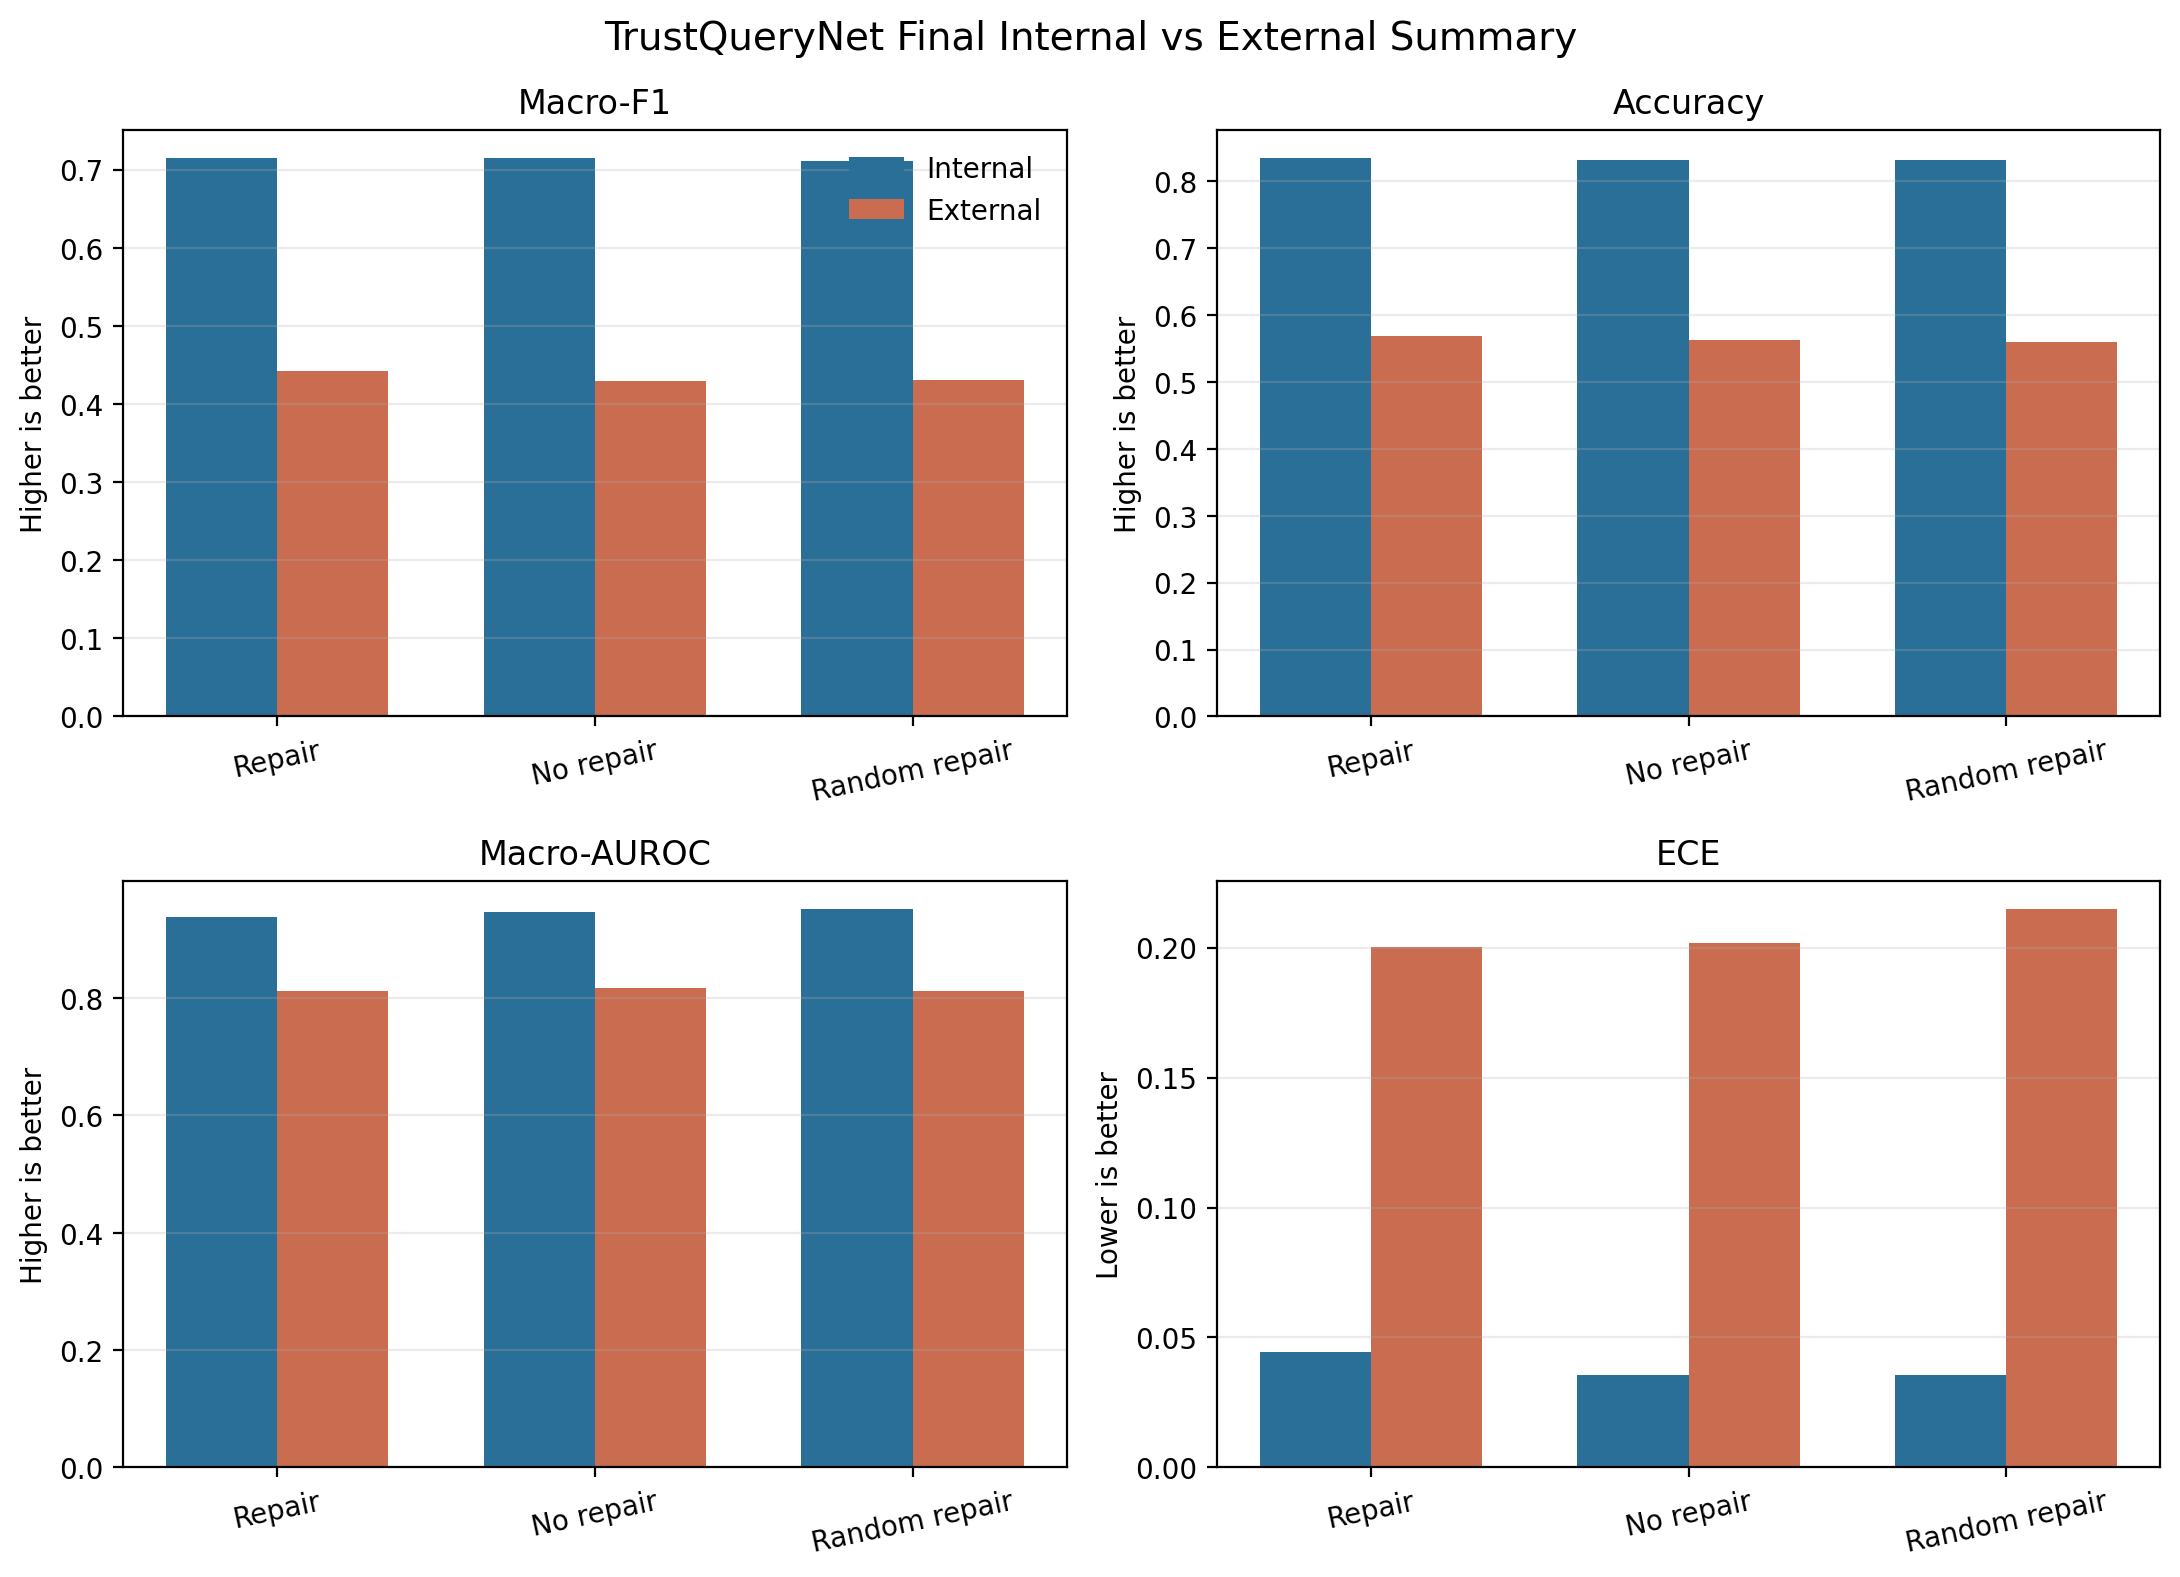
\includegraphics[width=0.92\linewidth]{paper_figures/internal_external_summary.png}
\caption{Final internal-vs-external summary across the three main operational settings. Bars show multiseed means for calibrated macro-F1, accuracy, macro-AUROC, and ECE. Internal point performance remains strong, but all variants degrade substantially under external shift.}
\label{fig:summary}
\end{figure}

\begin{figure}[ht]
\centering
\begin{minipage}{0.49\linewidth}
\centering
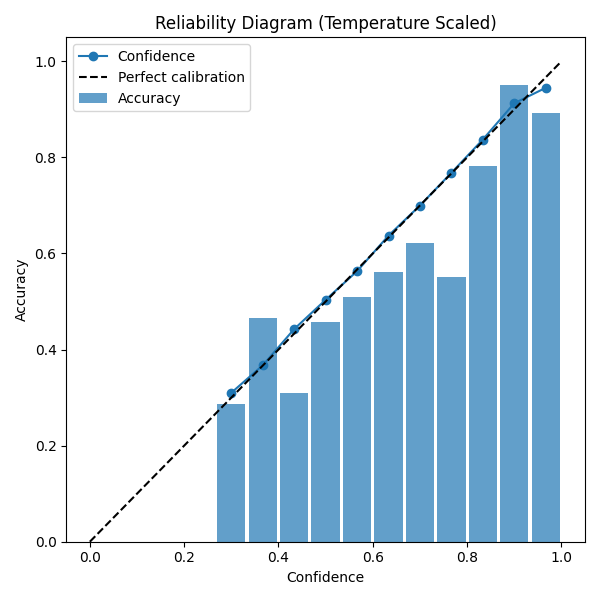
\includegraphics[width=\linewidth]{paper_figures/internal_reliability_calibrated.png}

\small (a) Internal calibrated reliability
\end{minipage}
\hfill
\begin{minipage}{0.49\linewidth}
\centering
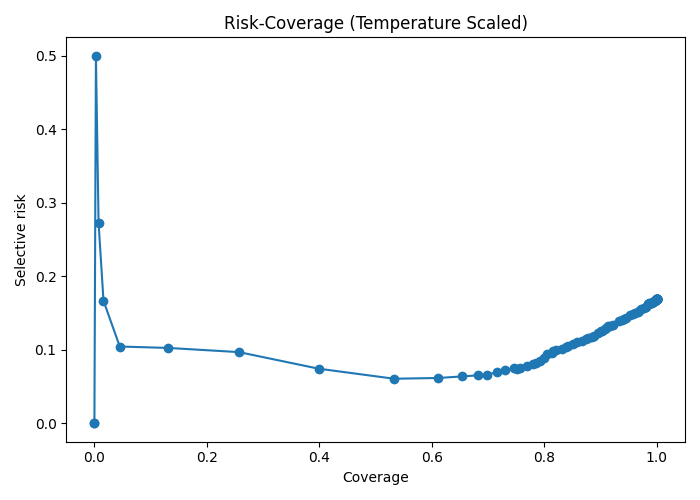
\includegraphics[width=\linewidth]{paper_figures/internal_risk_coverage_calibrated.png}

\small (b) Internal calibrated risk-coverage
\end{minipage}
\caption{Representative internal repair plots from \texttt{seed-72}, selected as the seed whose calibrated macro-F1 is closest to the repair multiseed mean. The panel is qualitative only and is not used for statistical comparison.}
\label{fig:internal-plots}
\end{figure}

\subsection{Noisy-label anchors}

\begin{table}[ht]
\centering
\resizebox{\textwidth}{!}{
\begin{tabular}{lccccccc}
\toprule
Setting & Accuracy & Macro-F1 & ECE & Macro-AUROC & AURC & Coverage@0.5 & Risk@0.5 \\
\midrule
Repair & $0.8350 \pm 0.0059$ & $0.7152 \pm 0.0216$ & $0.0445 \pm 0.0090$ & $0.9382 \pm 0.0133$ & $0.0728 \pm 0.0186$ & $0.9525 \pm 0.0074$ & $0.1428 \pm 0.0054$ \\
Clean upper & $0.8521 \pm 0.0055$ & $0.7330 \pm 0.0288$ & $0.0389 \pm 0.0176$ & $0.9583 \pm 0.0076$ & $0.0502 \pm 0.0095$ & $0.9618 \pm 0.0107$ & $0.1306 \pm 0.0089$ \\
GCE no repair & $0.6774 \pm 0.0012$ & $0.1224 \pm 0.0122$ & $0.0268 \pm 0.0381$ & $0.5782 \pm 0.1279$ & $0.2399 \pm 0.1059$ & $0.9639 \pm 0.0626$ & $0.3044 \pm 0.0327$ \\
\bottomrule
\end{tabular}
}
\caption{Noisy-label anchors and baseline comparisons. Repair is reported across five seeds; the clean upper bound and GCE anchor are reported across the shared three-seed subset.}
\label{tab:anchors}
\end{table}

The clean upper bound shows moderate remaining headroom, while the generalized cross-entropy baseline fails dramatically under the chosen noisy-label regime. This negative result is important: robust-loss substitution is not automatically beneficial in this setting.

\subsection{External validation}

\begin{table}[ht]
\centering
\resizebox{\textwidth}{!}{
\begin{tabular}{lccccccc}
\toprule
Setting & Accuracy & Macro-F1 & ECE & Macro-AUROC & AURC & Coverage@0.5 & Risk@0.5 \\
\midrule
Repair external & $0.5692 \pm 0.0145$ & $0.4427 \pm 0.0117$ & $0.2000 \pm 0.0253$ & $0.8125 \pm 0.0180$ & $0.2804 \pm 0.0299$ & $0.8526 \pm 0.0230$ & $0.3805 \pm 0.0228$ \\
No repair external & $0.5630 \pm 0.0078$ & $0.4288 \pm 0.0123$ & $0.2016 \pm 0.0123$ & $0.8168 \pm 0.0154$ & $0.2749 \pm 0.0183$ & $0.8498 \pm 0.0264$ & $0.3838 \pm 0.0073$ \\
Random repair external & $0.5591 \pm 0.0203$ & $0.4311 \pm 0.0328$ & $0.2149 \pm 0.0395$ & $0.8114 \pm 0.0337$ & $0.2905 \pm 0.0669$ & $0.8654 \pm 0.0383$ & $0.3964 \pm 0.0269$ \\
\bottomrule
\end{tabular}
}
\caption{External validation on the official ISIC 2019 test set, reported as calibrated test metrics (mean $\pm$ std) across five seeds.}
\label{tab:external-main}
\end{table}

All methods degrade sharply on ISIC 2019 relative to internal HAM10000 evaluation. Repair remains modestly ahead of the two comparison baselines on external accuracy and macro-F1, but it does not dominate all trust metrics. The overall lesson is not that repair solves external robustness, but that even modest internal gains must be interpreted cautiously under shift.

The external seed-paired comparisons remain modest. On calibrated macro-F1, repair exceeds no repair by $0.0139$ (95\% CI $[-0.0044, 0.0281]$, exact sign-flip $p=0.1875$) and random repair by $0.0117$ (95\% CI $[-0.0097, 0.0329]$, $p=0.4375$). These deltas are directionally favorable for repair but are not strong evidence of a large or universal external trustworthiness gain.

\begin{figure}[ht]
\centering
\begin{minipage}{0.49\linewidth}
\centering
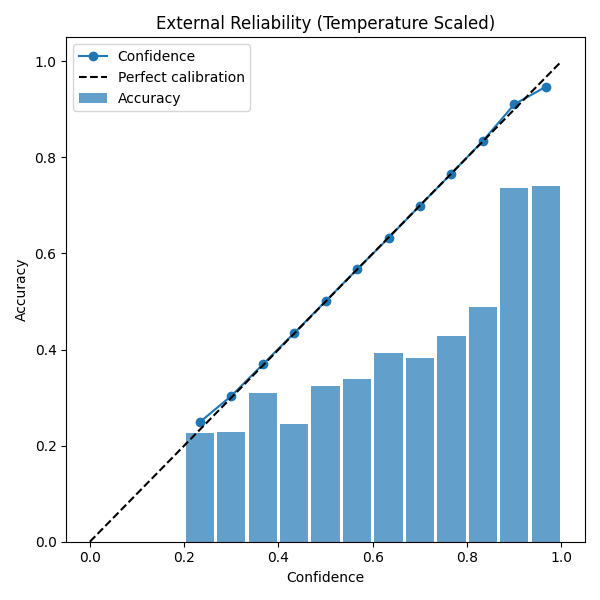
\includegraphics[width=\linewidth]{paper_figures/external_reliability_calibrated.png}

\small (a) External calibrated reliability
\end{minipage}
\hfill
\begin{minipage}{0.49\linewidth}
\centering
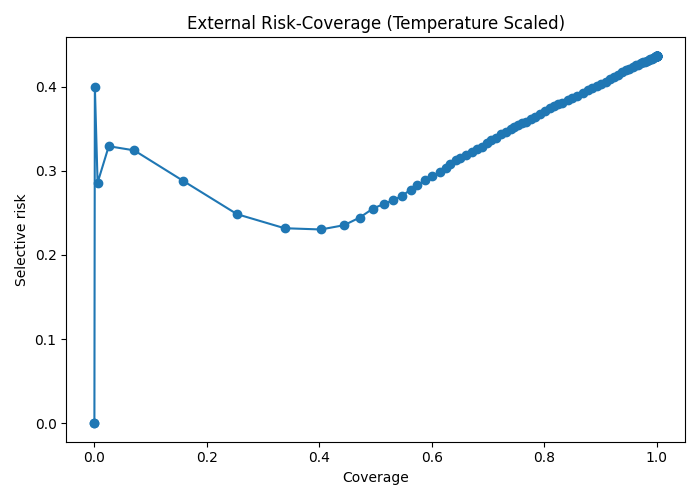
\includegraphics[width=\linewidth]{paper_figures/external_risk_coverage_calibrated.png}

\small (b) External calibrated risk-coverage
\end{minipage}
\caption{Representative external repair plots from \texttt{seed-72}. The visual shift from the internal curves is consistent with the large external degradation in accuracy, macro-F1, ECE, and AURC. As in Figure~\ref{fig:internal-plots}, the panel is qualitative and the representative seed is recorded in the figure manifest.}
\label{fig:external-plots}
\end{figure}

\subsection{Overlap audit}

The overlap audit found 10{,}015 HAM10000 samples, 6{,}191 mapped ISIC 2019 external samples, zero exact duplicate images, and 14{,}185 perceptual-hash candidate pairs at dHash $\leq 4$. The zero exact matches are the key integrity result. The perceptual-hash list is a deliberately coarse candidate screen for manual or secondary review and should not be interpreted as confirmed overlap or confirmed leakage.

\section{Discussion}

The final evidence supports a restrained but useful conclusion. Budgeted trusted-label repair is not a universally dominant intervention in this setting. It yields only a modest advantage over no-repair and random-repair baselines in point performance, while other trust metrics remain mixed. This is exactly why the stronger baseline suite matters: without random repair and no repair, it would have been easy to overstate the value of repair.

The external findings are the most important part of the paper. Internal HAM10000 performance is strong for all competitive variants, but all of them degrade substantially on ISIC 2019. That drop is not a side note; it is the central trustworthy-ML result. Similarly, post-hoc calibration learned in-distribution does not remove external confidence fragility, echoing broader warnings about uncertainty evaluation under distribution shift \citep{combalia2022isic2019,ovadia2019uncertainty}.

The paper is therefore strongest when framed as an externally validated experimental study rather than a method paper. Its contribution is evidence: which interventions remain competitive, which fail, and how internal trust signals do or do not transfer externally. In practical terms, the study argues against two common over-interpretations: that a small internal macro-F1 gain implies materially safer external behavior, and that post-hoc calibration fitted in-distribution is sufficient evidence of trustworthy deployment readiness.

\section{Limitations}

\begin{itemize}
  \item The label-corruption process is simulated and class-dependent; it is not estimated from observed expert disagreement patterns.
  \item The repair protocol is simulated oracle supervision, not prospective expert annotation or a clinician-in-the-loop workflow.
  \item External validation is limited to one official external benchmark and one fixed taxonomy-mapping choice.
  \item Seed-paired statistical reporting is available for the prespecified main comparisons, but its resolution is limited by five-seed main runs and a three-seed GCE anchor.
  \item Perceptual-hash overlap candidates were not exhaustively adjudicated manually, so only the zero exact-duplicate result is definitive.
  \item No clinician reader study, workflow study, or deployment evaluation is included.
  \item The work is comparative and evaluative; it does not introduce a new learning algorithm.
\end{itemize}

\section{Conclusion}

TrustQueryNet is now a credible applied research package for trustworthy dermatoscopic classification under noisy supervision. The final evidence shows that internal gains do not guarantee external trustworthiness, that trusted-label repair must be judged against strong baselines including random repair, and that robust-loss substitution can fail outright in this regime. These are publishable applied findings when presented honestly and with external validation.

\bibliographystyle{unsrtnat}
\bibliography{references}

\end{document}
